\chapter{Development} % (fold)
\label{chap:development}

\section*{Reader Guidance} % (fold)
\label{sec:dev_reader_guidance}
This chapter describes in detail the concepts behind the results of this
thesis. In contrast to Chapter~\ref{chap:api}, it is not a matter of defining
the whole API of this library in breadth but of presenting the background and
considerations understandably. \\
The first part of this chapter describes how iterables work in JavaScript and
what a sequence is in the context of this project. Then it shows how to use the
Decorator Pattern to build functions available to all iterables. \\ 
The second part shows how programs can be better structured using approaches
found in functional programming languages. These approaches allow the adoption
of abstract and strong concepts from Haskell to JavaScript. \\ 
The final part is devoted to testing - how to test different functions with
similar requirements safely and why tests based on invariants are helpful.
% section Reader Guidance (end)
\section{Sequence and Iterable in General}
\label{sec:Sequence and Iterable in General}
This section explains the concept of iterable objects and shows how to create 
them. Sequence is one such implementation. It illustrates how the benefits of 
iterators are utilized in a specific implementation using illustrations and 
explanations.

\subsection{What is an Iterator?}
\label{sub:What is an Iterator?}
Iterators are a common notion in computer science. An iterator is a mechanism 
to access elements of any data structure. It uses a function call to return the 
next element and either act on a data structure in memory or compute the 
elements when queried. Iterators are an essential part of this work. Therefore, 
the fundamentals are essential to understand, and the following sections cover
the topic in depth.

% \subsection{Iteration Protocols in JavaScript}
\subsection{Exploring the Meaning Of Protocols}
\label{sub:Exploring the Meaning Of Protocols}
In JavaScript, an iterator is an object that implements the JavaScript iterator
and iterable protocols \cite{mdn_iteration_2023}
(henceforth called JS iteration protocols). An iterator
has the characteristic of only iterating once across a collection of items.
After that, the iterator is exhausted, and the following operations will be
performed on a new instance.

\subsubsection{The Iterable Protocol}
\label{subsub:The Iterable Protocol}
An object is an iterable according to the JS iterable protocol if it has a
property with the name |[Symbol.iterator]|. Thus, such an object is of type
|Iterable<T>| which defines its iteration behavior.
All objects in JavaScript that have this property can be processed using 
destructuring and |for...of| loop. 
The sample code for defining a property named |[Symbol.iterator]| is shown
in Listing \ref{lst:iterable_protocols}. The value of this property is a
function which has to follow the iterator protocol.

\begin{lstlisting}[
  style=ES6, 
  caption=Iterable protocol,
  label={lst:iterable_protocols}
  ]
  return {
    [Symbol.iterator]: () => {
      return { next: next };
    }
  }
\end{lstlisting}

\subsubsection{The Iterator Protocol}
\label{subsub:The Iterator Protocol}
This protocol defines the structure of the iterator object. Invoking the 
|[Symbol.iterator]| property obtains such an object. These objects must 
implement a function next, which defines how and which values are returned 
when iterating.
Each iteration calls the function |next|. |next| returns an object, which must
have two properties according to the iterator protocol: |value| and |done|.
Therefore, the property |value| contains the current value of the iteration,
while |done| represents the information on whether the end of the iteration has 
been reached. The following code \ref{lst:iterator_protocol} shows a simple 
example implementation. Each call on |next| returns an object with the |value| 
1, and the iteration is never finished. 

\begin{lstlisting}[
  style=ES6, caption=Iterator protocol,
  label={lst:iterator_protocol}
  ]
  const next = () => {
    return { done: false, value: 1 };
  };
\end{lstlisting}

\subsubsection{Creating Iterables}
\label{subsub:Creating Iterables}
By combining the two protocols, the result could look like listing
\ref{lst:protocols}. In listing \ref{lst:protocols}, the constructor 
|SampleIterable| on line 1 wraps the two previously
defined implementations of the protocols. Objects from this constructor are now
iterables. It has the type |Iterable<Number>| because the return value from the
iterator is one.

\begin{lstlisting}[
  style=ES6, caption=Iterable and iterator protocol,
  label={lst:protocols}
  ]
 const SampleIterable = () => {

  const next = () => {
    return { done: false, value: 1 };
  };

  return {
    [Symbol.iterator]: () => {
      return { next: next };
    }
  }
};
\end{lstlisting}

Since |SampleIterator| follows the JS iterator protocols it is now possible to 
construct iterable objects. Built-in language features like |for..of| and 
destructuring (|...|) can now process these objects. However, beware in this 
case. This would lead to an infinite loop because the property done never 
becomes true. We will see examples with non-endless iterators later in this. 
Nevertheless, for now, the focus here is on the protocols. Therefore this 
example will be sufficient at this point.
\newline
Such protocols make it possible to iterate your customized objects and
collections. This opens new possibilities. Various programming tasks can be 
solvable differently, probably more straightforwardly.\newline
There are already some languages built-in iterable in JavaScript. Array and
HTML Collections are probably the most prominent of these.

\subsection{Types of Iterables}
\label{sub:Types of Iterables}
Previously we saw a distinction between 
iterables~\ref{subsub:Creating Iterables} and 
iterator~\ref{subsub:The Iterator Protocol}. These abstractions also have their 
types. Listing \ref{lst:iterable_types} shows an excerpt of the relevant types.

\begin{lstlisting}[
  style=ES6, caption=Types of iterables,
  label={lst:iterable_types}
  ]
// lib.es2015.iterable.d.ts

interface Iterable<T> {
    [Symbol.iterator](): Iterator<T>;
}

interface Iterator<T, TReturn = any, TNext = undefined> {
    next(...args: [] | [TNext]): IteratorResult<T, TReturn>;
    return?(value?: TReturn): IteratorResult<T, TReturn>;
    throw?(e?: any): IteratorResult<T, TReturn>;
}

type IteratorResult<T, TReturn = any> = IteratorYieldResult<T> 
                                      | IteratorReturnResult<TReturn>;

interface IteratorReturnResult<TReturn> {
    done: true;
    value: TReturn;
}
\end{lstlisting}

An iterable is of type |Iterable<T>|, whereas the object returned by the property
|[Symbol.Iterator]| is of type |Itertator<...>|. As shown in listing
\ref{lst:iterable_types}, an iterator is required to have a property next. 
This is the function that returns values when iterating. These values must be 
of type |IteratorResult<...>|, defined on line 8 of listing 
\ref{lst:iterable_types}. |IteratorResult<...>| itself is defined to return an 
object of type |ItereratorReturnResult<...>|. This object contains the actual 
values we want to work with. Examining these types illustrates how JavaScript's 
iterators have been built and reveal that some objects are nested within each
other. There is a reason for this. We will get to the roots of these in
chapter~\ref{sub:Stateful Decorating}.

\subsection{Building custom Series of Data}
\label{sub:Building custom Series of Data}
The last chapter has shown how to make an object iterable. By exploring the 
protocols discussed so far, this chapter showcases the ability to create 
powerful concepts. Previously, an endless iterator that generates only ones 
served as an illustration. The goal is to create a constructor that can 
produce arbitrary data series.

\subsection{Sequence - The Name of connected Data}
\label{sub:Sequence - The Name of connected Data}
As is often the case in computer science, finding the proper names is one of 
the hardest things in programming sustainable and robust code. Various arguments 
have contributed to the fact that the constructor for creating any series is 
called "Sequence". First, sequences are not conventional lists known from other 
programming languages. However, it must be clear from the name that it is about 
connected data. Second, it carries a small risk of introducing new names and
thus discourages users. However, we chose the name because it was important not
to make false assumptions about what we were working with. 
\newline
The nice thing about the objects generated by Sequence compared to
conventional lists is that one has the feeling of handling large 
amounts of data arbitrarily. In reality, however, only a minimum of memory is 
needed because the subsequent elements are not yet in memory.

\subsection{Everything a Sequence needs}
\label{sub:Everything a Sequence needs}
Defining a Sequence of data requires specifying three essential points:
\begin{enumerate}
  \item{A fixed starting value for the Sequence} 
  \item{A function to calculate the next element based on its predecessor} 
  \item{A function to determine if the Sequence has reached its end} 
\end{enumerate}
These three elements define the Sequence and are passed as arguments, 
see listing \ref{lst:sequence} line~\ref{line:seq_args}.
To keep the focus on the core elements of the Sequence, some functionality in 
listing \ref{lst:sequence} is discussed later. The |next| function, explained in 
the Iterator Protocol section~\ref{subsub:The Iterator Protocol}, 
is on lines~\ref{line:start_protocol}~-~\ref{line:end_protocol}. It contains the 
logic to return the next object of an iteration. First, it uses |untilFunction| 
to check if the Sequence has finished. If this is not the case, the
|incrementFunction| calculates the next element and returns it.

\begin{lstlisting}[
  style=ES6, 
  caption=Parts of Sequence,
  label={lst:sequence}
  ]
// Sequence.js
const Sequence = (start, untilFunction, incrementFunction) => {*'\label{line:seq_args}'*

  const iterator = () => {
    let value = start;
    /**
     * @template _T_
     * Returns the next iteration of this iterable object.
     * @returns { IteratorResult<_T_, _T_> }
     */
    const next = () => {*'\label{line:start_protocol}'*
      const current = value;
      const done = !untilFunction(current);
      if (!done) value = incrementFunction(value);
      return { done, value: current };*'\label{line:end_protocol}'*
    };

    return { next };
  };

  return createMonadicSequence(iterator);
};
\end{lstlisting}


\subsubsection{Using a Sequence}
\label{subsub:Using a Sequence}
Listing \ref{lst:even-sequence} shows the definition of a sequence of even 
numbers smaller than ten and how to use it. 
\begin{lstlisting}[
  style=ES6, 
  caption=Sequence over the even numbers,
  label={lst:even-sequence}
  ]
const startValue        = 0;
const untilFunction     = x => x < 10;
const incrementFunction = x => x + 2;

const seq = Sequence(startValue, untilFunction, incrementFunction);

for (const elem of seq) {
  console.log(elem);
}

// => Logs '0, 2, 4, 6, 8' *'\label{line:demo_output}'*
\end{lstlisting}

The |for..of| loop iterates over each
element until |done| is true. Meanwhile, |console.log| writes the elements out 
to the console. Line~\ref{line:demo_output} shows the output produced.
\newline

Now, we discussed the ability to generate arbitrary sequences of data. However, 
just creation is often inadequate as there is a need to manipulate the data or 
introduce additional levels of abstraction. In the upcoming chapter, we will 
delve into processing such sequences.

\section{Decorating Sequences}
\label{sec:Decorating Sequences}
This chapter explores how to process Sequences by implementing the Decorator 
Pattern and effectively managing Sequence state. Discover powerful techniques 
to enhance Sequence functionality and manipulate data.

\subsection{Decorator Pattern}
\label{sub:Decorator Pattern}
% TODO Zitat von Gang of four
Let us look at the Decorator Pattern~\cite{} to understand the content of the following sections.
In object-oriented programming, the decorator pattern is a widely used concept. 
An object is decorated, as the name implies. As a result, an outer object refers 
to an inner object, and both implement the same interface. As a result, the 
outer object forwards requests to the inner one. It modifies the calls on 
demand to manipulate or decorate the functionality of the inner one. Figure
\ref{} shows how a decorator forwards the receiving calls and transfers the
answer back to the client.

\usetikzlibrary{calc,positioning,arrows}
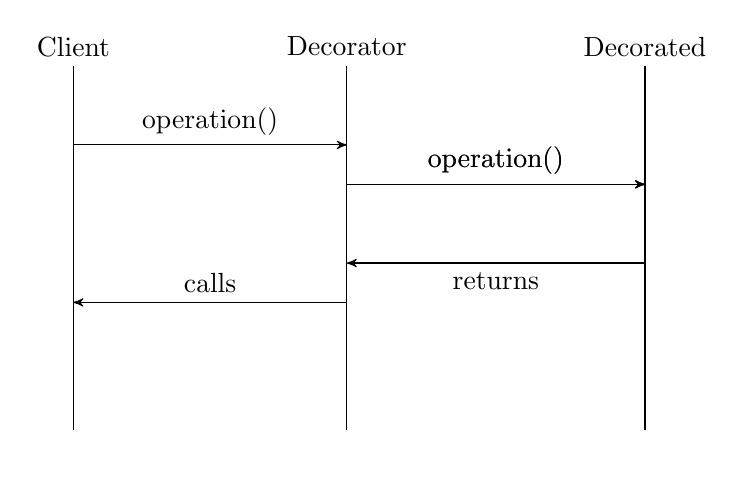
\begin{tikzpicture}[node distance=2cm,auto,>=stealth']
  \node[] (Decorated) {Decorated};
  \node[left = of Decorated] (Decorator) {Decorator};
  \node[left = of Decorator] (Client) {Client};
  \node[below of=Decorated, node distance=5cm] (Decorated_ground) {};
  \node[below of=Client, node distance=5cm] (Client_ground) {};
  \node[below of=Decorator, node distance=5cm] (Decorator_ground) {};
  %
  \draw (Client) -- (Client_ground);
  \draw (Decorated) -- (Decorated_ground);
  \draw (Decorator) -- (Decorator_ground);
  \draw[->] ($(Client)!0.25!(Client_ground)$) -- node[above,scale=1,midway]{operation()} ($(Decorator)!0.25!(Decorator_ground)$); 
  \draw[->] ($(Decorator)!0.35!(Decorator_ground)$) -- node[above,scale=1,midway]{operation()} ($(Decorated)!0.35!(Decorated_ground)$); 
  \draw[->] ($(Decorator)!0.35!(Decorator_ground)$) -- node[above,scale=1,midway]{operation()} ($(Decorated)!0.35!(Decorated_ground)$); 
  \draw[->] ($(Decorated)!0.55!(Decorated_ground)$) -- node[below,scale=1,midway]{returns} ($(Decorator)!0.55!(Decorator_ground)$);
  \draw[->] ($(Decorator)!0.65!(Decorator_ground)$) -- node[above,scale=1,midway]{calls} ($(Client)!0.65!(Client_ground)$); 
\end{tikzpicture}

The Decorator Pattern is often used in object-oriented programming languages 
because it adds additional functionality to an object at runtime. It is also 
possible to add extended functionality to a single object of a class. In the 
following, we will see how to exploit this to manipulate and change an Iterable.

\subsection{Processing Sequences}
\label{sec:Processing Sequences}
We use exactly that decorating approach to process Sequences further. 
The goal is to find a way to manipulate sequences so that they can solve 
complex problems. With many other programming languages it is possible to write
programs in this way. Lists and operations on lists solve numerous problems in 
computer science. This way of programming has the advantage that the structure 
of the code is declarative. This code is easier to understand and extend.

\subsubsection{Manipulate Iteratbles with Functions}

In the following, |map| serves as a representative for any function of the
Sequence library.
Listing~\ref{lst:impl_map} shows how |map| processes a Sequence. 
For this, we use the Decorator approach just mentioned. To keep the example 
simple, on Line~\ref{line:seq_definition} a client calls the map function with a Sequence of numbers. But it
could process any kind of iterables.
\newline
On line~\ref{line:args}, the function signature shows that a client can invoke 
|map| with two arguments: a mapper-function capable of processing an element of
an iterable and an iterable itself. An iterable must adheres to the protocol outlined in 
Section~\ref{subsub:The Iterable Protocol}. As a result, map can process 
Sequences, Arrays or any other iterable. 

\begin{lstlisting}[
  style=ES6, 
  caption=Implementation of map,
  label={lst:impl_map}
  ]
const map = mapper => iterable => { *'\label{line:args}'*
*'\label{line:state_iterable}'*
const mapIterator = () => {
   const inner = iteratorOf(iterable);*'\label{line:state_iterator}'*
   let mappedValue;
 
   const next = () => {
     const { done, value } = inner.next();*'\label{line:inner_next}'*
     if (!done) mappedValue = mapper(value);
 
     return { /**@type boolean */ done, value: mappedValue }
   };
 
   return { next };
  };
 
  return createMonadicSequence(mapIterator);
};

const sequence = Sequence(0, x => x < 10, x => x++);*'\label{line:seq_definition}'*
const mapped   = map(x => x * 2)(sequence);*'\label{line:obj_mapped}'*
\end{lstlisting}

Because map decorates iterables, |map| also returns an object of type Iterable. 
We define this object on line~\ref{line:obj_mapped} as mapped. 
Consequently, |map| also has a next function. Since the Iterable protocol 
specifies only this single function, it is the only one that must be externally 
callable. The object mapped now forwards function calls of the next function to 
the inner iterable, on line~\ref{line:inner_next}. The mapper function then processes the 
result and returns it.

\subsection{Benefits form the Decorater Approach}
\label{sub:Benefits form the Decorater Approach}
This section discusses the benefits and consequences of using the Decorator Pattern 
to implement the Sequence Library.

\subsubsection{Standalone Functions}
\label{subsub:Standalone Functions}
In an object-oriented approach, the Sequence object defines the functions to 
process the elements. Functions are available by using dot notation. Similar to 
Java implements the Stream API. However, with the approach of programming the 
functions independently, there are three significant advantages:
\begin{enumerate}
  \item {Strict adherence to the open-close principle. Changes to a function do
      not affect the implementation of Sequence. Also, extensions to the 
      Sequence library do not affect existing code.
    }
  \item{Adherence to the single responsibility approach. The Sequence 
      constructor has only the task of creating a sequence. Mapping the
    elements of a sequence is not its responsibility.
  }
  \item{Easy scalability is guaranteed. It is very straightforward to add new 
    functionality from the outside.
  }
\end{enumerate}

Due to the independent implementation of the functions, the last parameter can 
be the iterable object. The functions therefore define the parameters in curried 
style. Therefore, it is possible to benefit from eta-reduction in different
situations.

\subsection{Stateful Decorating}
\label{sub:Stateful Decorating}
A state is present as soon as functions decorate iterables or implement 
additional functionalities. This chapter is about where the functions implement 
this state and which consequences this implies.

There are two possible locations to bring state in. First into the 
closure scope of the surrounding function of the iterator, in
listing~\ref{lst:impl_map} on line~\ref{line:state_iterable} in the following 
referred as iterable state. Second into the closure scope of 
the function which is returned from the |[Symbol.iterator]| property, on
line~\ref{line:state_iterator}, reffered to iterator state. Both variants are possible and will 
be discussed in the following.

\section{Iterables Everywhere}
\label{sec:Iterables Everywhere}
This chapter concerns the implications of the previous findings for other
data structures.
Some immutable collections are already implemented in the Kolibri Web Ui
Toolkit~\cite{kolibri}. The Pair example demonstrates the advantages of 
iterating existing implementations in the following section.

\subsection{Making immutable Data Structures iterable}
\label{sub:Making immutable Data Structures iterable}
In the following, we will examine the implementation of immutable Pair. 
There are no immutable collections by default in JavaScript, so you have to 
build them yourself. The Kolibri Web Ui Toolkit already implements some 
immutable collections. Listing~\ref{lst:pair_non_iterable} shows how to create and use a Pair.

\begin{lstlisting}[
  style=ES6, 
  caption=Immutable Pair,
  label={lst:pair_non_iterable}
  ]
/** *'\label{line:start_pair_type}'*
 * @typedef PairType
 * @type {  <_T_, _U_>
 *          (x: _T_)
 *       => (y: _U_)
 *       => (s: PairSelectorType<_T_, _U_>) => ( _T_ | _U_ ) 
 *      }
 */ *'\label{line:end_pair_type}'*
const pair = Pair(1)(2);

const one  = pair(fst);*'\label{line:fst_pair}'*
const two  = pair(snd);*'\label{line:snd_pair}'*

console.log(one + " " + two);
// => Logs '1 2'
\end{lstlisting}

The only way to make a Pair immutable is to build it from functions. The type 
signature on line~\ref{line:start_pair_type}~-~\ref{line:end_pair_type} shows 
that the first two arguments are arbitrary values. Pair stores these two values. 
Selector functions named |fst| on line~\ref{line:fst_pair} and |snd| on 
line~\ref{line:snd_pair} grant access to these values. However, it is not 
possible to change the values in the Pair.
Listing~\ref{lst:pair_non_iterable} shows that handling a Pair can be tedious. 
It would be great to use the built-in JavaScript language features to access 
the content of a Pair. 

\subsubsection{Iterable Pair}
\label{subsub:Iterable Pair}
Listing~\ref{lst:pair_iterable} demonstrates the implementation of an iterable 
Pair. Still, Pair operates only with functions. However, it additionally defines the
|[Symbol.iterator]| property.

\begin{lstlisting}[
  style=ES6, 
  caption=Iterable Pair,
  label={lst:pair_iterable}
  ]
const Pair = x => y => {
  /**
   * @template _T_, _U_
   * @type { PairSelectorType<_T_,_U_> }
   */
  const pair = selector => selector(x)(y);

  pair[Symbol.iterator] = () => [x,y][Symbol.iterator]();*'\label{line:pair_symbol_iterator}'*

  return pair;
};
\end{lstlisting}

Line~\ref{line:pair_symbol_iterator} shows that 
this property defines a function, which only returns the |[Symbol.iterator]| 
property of array. The array stores the values of the Pair. Thanks to this 
procedure, all iterable functions are now available to Pair. Also, the 
operators from the Sequence library supports now working with a Pair.
Listing~\ref{lst:handling_pair_iterable} shows the usage of the iterable Pair. 
Line~\ref{line:pair_destructuring} shows the deconstruction of a Pair in the same way as an array. 
This access option is more convenient than in Listing~\ref{lst:pair_non_iterable}. 
Line~\ref{line:show_pair} demonstrates the use of operations from the Sequence 
Library. |show| converts an iterable into a string, analogous to how |toString|
works.

\begin{lstlisting}[
  style=ES6, 
  caption=Working with iterable Pairs,
  label={lst:handling_pair_iterable}
  ]
const pair = Pair(1)(2);

const [one, two] = pair;*'\label{line:pair_destructuring}'*

console.log(show(pair));*'\label{line:show_pair}'*
// => Logs '[1,2]'
\end{lstlisting}

This has significant advantages because it is now possible to process different 
collections with the same abstractions. Therefore, the motivation is great to 
make all collections iterable.


\chapter{Modularizing Programs} % (fold)
\label{chap:Modularizing Programs}
This chapter explains how to break down programs and functions into small,
reusable pieces using lazy evaluation and higher-order functions. The start
shows how Haskell implements these concepts. The subsequent discussion covers
the application and limitations of these concepts in JavaScript before showing
how the Sequence library overcomes these limitations, providing valuable tools
for writing reliable and reusable code.

% chapter Modularizing Programs (end)
\section{Gluing Programs together} % (fold)
\label{sec:Gluing Programs together}
John Hughes argues that functional programming languages provide two extra ways
to better partition programs and easily combine them later. He refers to them
as "glues"~\cite[p.3]{hughes_why_1989}. These are, on the one hand,
higher-order functions and, on the other hand, lazy evaluation.
% subsection Gluing Programs together (end)

\subsection{Using these Glues in Haskell} % (fold)
\label{sub:Using these Glues in Haskel}

\subsubsection{Higher-order Functions in Haskell} % (fold)
\label{subsub:Higher-order functions Haskell}
Higher-order functions receive another function as arguments or produce a
function as a result. This concept is fundamental in Haskell, where the whole
program is a single function. The easiest way to understand higher-order
functions is to look at an example:

\begin{lstlisting}[style=Haskell, 
                  caption=Higher-order functions in Haskell, 
                  label={lst:hof_haskell}
]
double    = \x -> 2 * x
quadruple = \x -> 4 * x
doubles   = map double [1,2,3,4]
quads     = map quadruple [1,2,3,4]

print $ doubles ++ quads
-- Prints '[2,4,6,8,4,8,12,16]'
\end{lstlisting}

Listing~\ref{lst:hof_haskell} shows how higher-order functions work in Haskell.
This code is very reusable since |map| takes a function as an argument to
transform the values of a list.
% subsubsection Higher order functions Haskell (end)

\subsubsection{Lazy Evaluation} % (fold)
\label{subsub:Evaluation}
Lazy evaluation describes a concept where a program only evaluates as many
statements as required. This concept makes it possible to work with lists that
have an infinite amount of values. Again, an example explains the concept best:

\begin{lstlisting}[
  style=Haskell,
  caption=lazy evaluation in Haskell,
  label={lst:lazy_eval_haskell}
]
as = [1..]*'\label{line:lazy_eval_haskell_1}'*
doubles = map double as*'\label{line:lazy_eval_haskell_2}'*

print $ take 4 doubles *'\label{line:lazy_eval_haskell_3}'*
-- Prints '[2,4,6,8]'
\end{lstlisting}
Line~\ref{line:lazy_eval_haskell_1} of listing~\ref{lst:lazy_eval_haskell}
defines a list with infinite values. Then the function |double|, defined in the
previous listing ~\ref{lst:hof_haskell}, is applied to this list. As the list
has infinite elements, eagerly evaluating it would take forever. But since
Haskell evaluates its statements lazily, nothing happens on
line~\ref{line:lazy_eval_haskell_2}. Haskell applies |double| not before line
~\ref{line:lazy_eval_haskell_3}, where |print| evaluates a part of the list (the
first four elements). Even then, Haskell exclusively uses |double| on those
four elements.\\
More theoretically, when applying the function $f$ to $g(x)$, $g$ produces only
as much output as $f$ actually needs. Therefore, working with large data sets
becomes much more convenient and faster. Suppose the elements in a list are
generated with a rule (as with list comprehensions or generators). Then lazy
evaluation brings excellent advantages: The whole list will never materialize
in the memory, only the current value. So you don't have to worry about what
happens when large amounts of data are processed. \\ Using these two concepts,
building large programs consisting of small parts is much easier.

% subsubsection Lazy evaluation (end)
% subsection Using the glues in Haskell (end)

\subsection{Using these Glues in JavaScript} % (fold)
\label{sub:Using these Glues in JavaScript}

\subsubsection{Higher-Order Functions in JavaScript} % (fold)
\label{subsub:Higher Order Functions in JavaScript}
Higher-order functions in JavaScript work similarly as they do in Haskell.
Transferring listing~\ref{lst:hof_haskell} to JavaScript results in the
following:

\begin{lstlisting}[
  style=ES6,
  caption=Higher-order functions in JavaScript,
  label={lst:hof_in_js}
]
const double    = x => 2 * x;
const quadruple = x => 4 * x;
const doubles   = [1,2,3,4].map(double);
const quads     = [1,2,3,4].map(quadruple);

console.log(doubles.concat(quads));
// => Logs '2, 4, 6, 8, 4, 8, 12, 16'
\end{lstlisting}
% subsubsection Higher Order Functions in JavaScript (end)

\subsubsection{Eager Evaluation in JavaScript} % (fold)
\label{subsub:Eager Evaluation in JavaScript}

% subsubsection Lazy Evaluation in JavaScript (end)
It becomes less intuitive when it comes to lazy evaluation in JavaScript:
JavaScript does not know this concept when working with its in-built arrays.
Mapping over an array producing a side effect can shed some light on this:

\begin{lstlisting}[
  style=ES6,
  caption=JavaScript evaluates eagerly,
  label={lst:js_eagerly_eval}
]
const as     = [1,2,3,4,5];
const bs     = [];
const mapped = as.map(x => {
  bs.push(x);
  return 2*x;
});

console.log(mapped.slice(0,4));
// => Logs '2, 4, 6, 8'
console.log(bs);
// => Logs '2, 4, 6, 8, 10'
\end{lstlisting}

Listing ~\ref{lst:js_eagerly_eval} clarifies that even though the program only
uses the first four elements of the array, it traverses each element using the
passed function. This gets clear because the array |bs| contains all array
elements of |as| and not just its first four.

\subsubsection{Lazy Evaluating Iterables} % (fold)
\label{subsub:Lazy Evaluate Iterables}

% subsubsection Lazy Evaluate Iterables (end)
The eager evaluation of JavaScript is a significant limitation. Fortunately,
JavaScript can emulate this laziness using the JS iteration protocols, which
section ~\ref{sec:Iterables in General} describes.

With the use of the Sequence library, it is possible to rewrite the JavaScript
code of listing~\ref{lst:js_eagerly_eval} lazily:

\begin{lstlisting}[
  style=ES6,
  caption=Lazy evaluation in JavaScript,
  label={lst:lazy_eval_js}
]
const as     = [1,2,3,4,5];
const bs     = [];
const mapped = map(x => {
  bs.push(x);
  return 2*x;
})(as);

console.log(...take(4)(mapped));
// => Logs '2, 4, 6, 8'
console.log(bs);
// => Logs '1, 2, 3, 4'
\end{lstlisting}
The first output is the same as in listing ~\ref{lst:js_eagerly_eval} - the
first four elements of the array |as| have been multiplied by 2. However, the
second output differs: the array |bs| now contains only four elements! So |map|
applied the passed function only to four initial array elements! This fact
proves that transforming arrays using the Sequence library happens lazily!\\
This works because the JS iteration protocols process element by element. The
iterator delivers the next element only if it is requested. If no further
elements are needed, it just stops iterating! \\
Iterators, therefore, decouple the termination condition (asking for another
element) from the loop body (generating/accessing the next element).

Furthermore, it is even possible to port the initial Haskell laziness
example defined in listing~\ref{lst:lazy_eval_haskell} to JavaScript:
\begin{lstlisting}[
  style=ES6,
  caption=Process infinite sequences in JavaScript,
  label={lst:inf_seq_js}
]
const seq     = Sequence(1, _ => true, x => x + 1);*'\label{line:inf_seq_js_1}'*
const doubles = map(double)(seq);

console.log(...take(4)(doubles));
// => Logs '2, 4, 6, 8'
\end{lstlisting}

If the code displayed in Listing~\ref{lst:inf_seq_js} were evaluated eagerly,
this would go on forever since line~\ref{line:inf_seq_js_1} defines a sequence
with infinite elements. \\ 

\subsection{Lazy Evaluation and Side Effects} % (fold)
\label{sub:Lazy Evaluation and Side Effects}
Decoupling the loop body and termination condition helps to consider these two
concepts separately. This split reasoning makes sense since they often do not
relate to each other. Why change the whole list of elements if the program only
uses the first five? In JavaScript, however, this thinking carries a danger
that cannot occur in pure functions like those used in Haskell. \\ 
The following listing~\ref{lst:side_effects_lazy_js} states the problem:

\begin{lstlisting}[
  style=ES6,
  caption=Side effects and lazy evaluation,
  label={lst:side_effects_lazy_js}
]
let i = 0;
const mapped = map(x => {
  i++;
  return 2 * x;
})([1,2,3,4]);

console.log(i);
// => Logs '0' i has not been incremented
console.log(...take(2)(mapped));
// => Logs '2, 4' 
console.log(i);
// => Logs '2' i has only been incremented two times
\end{lstlisting}

It is impossible to conclude from the length of the list how often a function
runs. Performing side effects in the loop body can lead to unexpected behaviour. 

It is tough to make assumptions about |i|, because:
\begin{itemize}
  \item |i| is only calculated when the program is evaluated
  \item It is impossible to predict what value |i| will have when the program
    finishes.
\end{itemize}
This example shows that lazy evaluation and side effects almost exclude each
other. Therefore, omitting side effects when working with lazy evaluation makes
sense. In Haskell, where the type system can exclude side effects per function
definition, this is not a problem. Since side effects often make a program
harder to understand, getting rid of it feels even more natural.
% subsection Lazy evaluation and side effects (end)

\section{Placing the Receiver at the End} % (fold)
\label{sec:Placing the Receiver at the End}
Compared to object-oriented programming languages, where the receiver of an
operation is always placed before the point (i.e., at the beginning), functions
in Haskell usually expect it as the last argument. If one sticks to this, it is
possible to give a new name to a partially applied (pre-configured)
function. Line~\ref{line:precon_fs_hs_1} of the following Haskell
listing~\ref{lst:precon_fs_hs} does precisely this and results in a reusable
pre-configured function (|doubleAll|) with a very descriptive name:
\begin{lstlisting}[
  style=Haskell,
  caption=Pre-configured functions in Haskell,
  label={lst:precon_fs_hs}
]
double    = \x -> 2 * x
doubleAll = map double --*'\label{line:precon_fs_hs_1}'* preconfigure map with the function double
as        = [1,2,3,4]
bs        = [5,6,7,8]

print $ doubleAll as ++ doubleAll bs
-- Prints '[2,4,6,8,10,12,14,16]'
\end{lstlisting}

This paradigm allows it also to link existing functions together using the |.|
(dot) operator:

\begin{lstlisting}[
  style=Haskell,
  caption=Function composition in Haskell,
  label={lst:fn_comp_hs}
]
-- "sum" sums up all elements in the list
doubleAndSum = sum . doubleAll

print $ doubleAndSum [1,2,3,4]
-- Prints '20'
\end{lstlisting}

Listing~\ref{lst:fn_comp_hs} links the functions |doubleAll| and |sum| to
create a new function applicable to any list with numerical values. This
concept makes the code very reusable.\\
Placing the receiver at the end is another powerful modularization
tool. Therefore, the Sequence library supports this kind of modularization.
Refactoring the initial example from listing~\ref{lst:hof_in_js}, which 
shows how higher-order functions work in JavaScript, results in the following:

\begin{lstlisting}[
  style=ES6,
  caption=Receiver before the point,
  label={lst:rec_bef_point}
]
// initial code
const double  = x => 2 * x;
const doubles = [1,2,3,4].map(double);

// refactored using plain JS
const doubleAll = receiver => receiver.map(double);
console.log(doubleAll([1, 2, 3, 4]));
// => Logs '2, 4, 6, 8'
\end{lstlisting}

Listing~\ref{lst:rec_bef_point} fixes this issue using a function that gets
the receiver as an argument. However, this is not very convenient. The Sequence
library provides a more elegant way to solve this:

\begin{lstlisting}[
  style=ES6,
  caption=Place the receiver at the end in JavaScript,
  label={lst:rcv_at_end_js}
]
const doubleAll = map(double);
\end{lstlisting}

The code of listing~\ref{lst:rcv_at_end_js} is not only less to type but also
more accurate when reading because the term |doubleAll = map(double)| says that
the pre-configured function |map(double)| gets a new name (|doubleAll|). No worrying about
parameter naming is needed here!
% subsubsection Placing the Receiver at the End (end)

\subsubsection{Conclusion} % (fold)
\label{subsub:modularizing_programs_conclusion}
Higher-order functions and lazy evaluation are powerful glues to compose
smaller parts into a more extensive program. Haskell provides a good reference for
this. In JavaScript, higher-order functions are familiar. However, it
offers less support for lazy evaluation - it eagerly evaluates arrays and their
operations. The Sequence library closes this gap because sequences work
similarly to Haskell lists. Thus, the Sequence library allows using both types
of glue in JavaScript.
% subsubsection Conclusion (end)

\chapter{Monads in JavaScript} % (fold)
\label{chap:Monads in JavaScript}
The first part of this section describes what contexts in Haskell are and how
Haskell wraps values in such contexts. "Maybe" serves as an example of this.
Implementing this example using JavaScript shows that such contexts are also
useful in other programming languages.\\
The second part then explains monads and describes how to implement them with JavaScript.
It also highlights the missing features of JavaScript to adopt
this concept exactly from Haskell and describes acceptable workarounds. Thus, it
is also possible to transform values in a context in JavaScript. The
last part shows what the monadic operations of the sequence look like.

\section{Wrapping Values in a Context} % (fold)
\label{sec:Wrapping values in a context}
In Haskell, you often work with values wrapped in a particular context. This
context can be, for example, a list. Nevertheless, this context can also be
another data structure, for instance, the polymorphic type |Maybe|. \\
For the context |Maybe| two implementations in Haskell co-exist:

% section Monads in JavaScript (end)
\begin{lstlisting}[
  style=Haskell,
  caption=The data type Maybe in Haskell,
  label={lst:maybe_hs}
]
-- defining the datatype Maybe
data Maybe a = Nothing | Just a
\end{lstlisting}

Listing~\ref{lst:maybe_hs} defines the datatype |Maybe|. Why is this useful?
Imagine you want to create a function |head| which returns the first value of
a given list. |head| is pretty simple to implement. But wait, what to do when
the list is empty? In object-oriented languages, one might return |null|. The
problem with this solution is that the user of |head| must remember that the
list can be empty, and thus the result of |head| can be |null|. This is very
error-prone.

That is where the new datatype |Maybe| comes in. |Maybe| allows describing
either the absence of a value or the value itself. The following
listing~\ref{lst:safe_head} defines a new function |safeHead|
(line~\ref{line:safe_head1}), which does precisely this - it returns |Just a|
with |a| containing the first value of the list when it is not empty
(line~\ref{line:safe_head2}) and |Nothing| otherwise (line~\ref{line:safe_head3}):

\begin{lstlisting}[
  style=Haskell,
  caption=Safely get the first element of a list,
  label={lst:safe_head}
]
-- a function which produces a Maybe:
safeHead :: [a] -> Maybe a *'\label{line:safe_head1}'*
safeHead (a:_) = Just a *'\label{line:safe_head2}'*
safeHead []    = Nothing *'\label{line:safe_head3}'*

printHead list = print $ case (safeHead list) of 
  Just val -> show val
  Nothing  -> "List was empty!"

printHead [1,2,3,4]
-- Prints '"1"'
printHead []
-- Prints '"List was empty!"'
\end{lstlisting}

The function |printHead| is forced to deal explicitly with the case when the passed
list is empty. When returning |null|, the user must remember to deal with
the case where there is no first element. Therefore, |Maybe| leads to improved safety.

\subsection{Doing the Same in JavaScript} % (fold)
\label{sub:Doing the same in JavaScript}
Listing~\ref{lst:maybe_js} defines the same type in JavaScript:
\begin{lstlisting}[
  style=ES6,
  caption=The data type Maybe in JavaScript,
  label={lst:maybe_js}
]
const Just    = x => _f => g => g(x);*'\label{line:maybe_js1}'*
const Nothing = f => _g => f(undefined);*'\label{line:maybe_js2}'*
\end{lstlisting}

So |Just| and |Nothing| are only functions! How could it be different in
functional programming? \\ 
Line~\ref{line:maybe_js1} defines the |Just| case:
|Just| takes a value |x| and two functions while not using the first function
at all. |Just| applies the second function to the initial value |x|. \\ 
|Nothing| looks very similar to |Just|, with the difference that it does not
receive a value. Furthermore, |Nothing| calls the second function at the end.\\ 
Now how to use this? Noticeably, |Just(value)| and |Nothing| have the same
structure: both receive two functions as arguments. Meaning they are
structurally the same. Listing~\ref{lst:js_safeHead} takes advantage of this
property to port the previous function |safeHead| to JavaScript:

\begin{lstlisting}[
  style=ES6,
  caption=safeHead implemented in JavaScript,
  label={lst:js_safeHead}
]
const safeHead = list => {
  const head = list[0];
  return (undefined === head) ? Just(head) : Nothing;
};

const printHead = list => {
  const maybeHead = safeHead(list);
  maybeHead *'\label{line:js_safeHead1}'*
    (_ => console.log("List was empty!")) // Nothing case
    (head => console.log(head));          // Just case *'\label{line:js_safeHead2}'*
};

printHead([1,2,3,4]);
// => Logs '1'
printHead([]);
// => Logs 'List was empty!'
\end{lstlisting}

Using the structural similarity of |Just(value)| and |Nothing|,
lines~\ref{line:js_safeHead1} to \ref{line:js_safeHead2} evaluate the result of
|safeHead|. The function |printHead|, therefore, works for both cases!
% subsubsection Doing the same in JavaScript (end)
% subsection Wrapping values in a context (end)

\section{Working with Values in a Context} % (fold)
\label{sec:Working with values in a context}
\subsection{Introducing fmap} % (fold)
\label{sub:Introducing fmap}
The example with maybe shows how values work in a context. Over time,
however, it can become tedious to keep making this distinction whether
it has a value. Therefore, Haskell offers a concept of working with values in a
context. The simplest way to work with the value using this concept is using
the function |fmap|. |fmap| knows how to execute a function for the value(s) in
a context. Listing~\ref{lst:fmap_maybe_hs} shows the usage of |fmap| for
maybe:

\begin{lstlisting}[
  style=Haskell,
  caption=fmap applied to Maybe,
  label={lst:fmap_maybe_hs}
]
double = \x -> 2 * x
print $ fmap double (Just 5)
-- Prints 'Just 10' 
print $ fmap double Nothing
-- Prints 'Nothing'
\end{lstlisting}

Similar to maybe, also lists describe such a context.
Listing~\ref{lst:hs_fmap_list} shows how |fmap| works on lists:

\begin{lstlisting}[
  style=Haskell,
  caption=fmap applied to a list,
  label={lst:hs_fmap_list}
]
print $ fmap double [1,2,3,4,5]
-- Prints '[2,4,6,8,10]'
\end{lstlisting}

Applying |fmap| to a list has the same result as applying |map| to a list.
Therefore, |fmap| is just a way to "map values".

% subsubsection Introducing fmap (end)
\subsection{Making a Context Monadic} % (fold)
\label{sub:Making a Context Monadic}
Haskell defines many other functions analogous to |fmap| to interact with
values in a context. So-called type-classes define these functions. In his book
"Programming in Haskell" Hutton describes type-classes like
\textcquote[p.~31]{hutton_pih_2016}{[...], a class is a collection of types
that support certain overloaded operations called methods. }\\ 
Some of these overloaded methods are more powerful than |fmap|. The following
section briefly overviews which operations a context must provide to be
considered monadic:

\begin{itemize}
  \item \textbf{Functor}: A context |f| is a |Functor| when it provides a function
|fmap|. |fmap| receives another function as an argument and applies it to the
value(s) in the context.\\
|fmap| signature: |fmap :: Functor f => (a -> b) -> f a -> f b|\\

\item \textbf{Applicative}: A context |f| is an |Applicative| when it is a |Functor|
and additionally provides two functions:
\begin{itemize}
  \item |<*>| (pronounced "app") receives another function as an
    argument wrapped in the same context and applies the unwrapped function to
    the value(s) in the context. \\
    |<*>| signature: |(<*>) :: Applicative f => f (a -> b) -> f a -> f b|
  \item |pure| receives a single argument and wraps it in the context. When
    describing |pure|, people often use the term lifting instead of wrapping.
    |pure| "lifts" a value into a context.\\
    |pure| signature: |pure :: Applicative f => a -> f a| \\
\end{itemize}
\item \textbf{Monad}: A context |m| is a |Monad| when it is an |Applicative|
  and additionally provides a function |>>=| (pronounced "bind"). |>>=| takes
  another function as an argument which, when applied to the value(s), again
  creates a value in the same context. So that the values are not nested twice
  in the context, |>>=| must resolve the inner context again. Therefore, |>>=|
  is like |fmap| but after mapping, the value(s) get flattened. Therefore, this
  operation is often also referred to as |flatMap|.\\
|>>=| signature: |(>>=) :: Monad m => m a -> (a -> m b) -> m b|\\
\end{itemize}

This list should briefly overview this hierarchy of type classes. For a little
deeper introduction to this topic, see, for example, ~\cite{monads_adit_2013}.
To really dive into it and see the rules each function follows, please see
\cite[Ch.~12]{hutton_pih_2016}.

% subsubsection Making a Context Monadic (end)
\subsubsection{Why using these Abstractions?} % (fold)
\label{subsub:Why using these Abstractions?}
These abstractions allow building general functions that can handle various
types. Listing~\ref{lst:hs_why_use_constraints} shows the function |doubleAll|
defined in listing~\ref{lst:fn_comp_hs} in a more general way, which is
applicable to lists and also maybes:

\begin{lstlisting}[
  style=Haskell,
  caption=Double the values in a context,
  label={lst:hs_why_use_constraints}
]
doubleAll :: (Functor f) => f Int -> f Int
doubleAll = fmap double

print $ doubleAll [1,2,3,4]
-- Prints '[2,4,6,8]'
print $ doubleAll $ Just 1
-- Prints 'Just 2'
\end{lstlisting}
Even though a list and a maybe have nothing in common, the same function can be
applied to both types! \\ 
\textit{Note:} Another example that makes use of these abstractions is JINQ,
which is described in the section~\ref{sec:Query different Data Structures}.
% subsubsection Why using these constraints? (end)
% subsection Working with values in a context (end)

\section{Monads in JavaScript} % (fold)
\label{sec:Monads in JavaScript}
Since monads are so good at handling values in a context, this concept is also
interesting for JavaScript. However, JavaScript has a weaker type system than
Haskell. Therefore, two important concepts can not be transferred to
JavaScript: 
\begin{enumerate}
  \item In Haskell, it is possible to force the type hierarchy hinted in
    section~\ref{sub:Making a Context Monadic}.
  \item Haskell can use its type system to determine a specific implementation
    for a function. The listing~\ref{lst:hs_fn_body} shows the binding of the
    function body to the name using the example of |fmap|:
    \begin{lstlisting}[
      style=Haskell,
      caption=Haskell determines the correct function body,
      label={lst:hs_fn_body}
    ]
-- The implementation for List is used
print $ fmap double [1,2,3,4]
-- The implementation for Maybe is used
print $ fmap double (Just 1)
    \end{lstlisting}
\end{enumerate}


Since it is not possible to implement these two concepts in JavaScript, a
different approach to these two problems is needed:
\begin{enumerate}
  \item Although it is possible to model a type hierarchy in JavaScript,
    enforcing it is impossible. Therefore, we created only one JSDoc type, the
    "|MonadType|". |MonadType| can be used as an interface, which defines all
    operations a monadic type must support.  
  \item Instead of inferring global functions automatically, the prototype of a
    monadic object gives access to them. \cite{mdn_prototype_2023}
\end{enumerate}
Section~\ref{sub:Using JSDoc to type monads} describes these workarounds in
detail.

\subsection{Which Operations fit JavaScript?} % (fold)
\label{sub:Which operations fit JavaScript?}
Since JavaScript works quite differently than Haskell, not all operations are
equally suitable to adopt. \\
The |MonadType| specifies the following operations:
\begin{itemize}
  \item |fmap|: Changing values inside a context is a typical pattern,
    also in JavaScript. Porting |fmap| to JavaScript brings many benefits.
  \item |pure|: At first sight, |pure| is a function that is not needed.
    However, it quickly became apparent that lifting an element into a context
    is often practical via an abstracted function. 
    \\ This is often the case when using |>>=|.
  \item |and (>>=)|: The |bind| operator allows access to the result of the last
    computation. |bind| is the only way to determine a new result depending on
    the previous result. \\ Since in JavaScript function names must not contain
    the special characters |>| and |=|, |>>=| cannot be used. |bind| is also
    already an existing function on every object. Using another term is
    required, therefore. We used the name |and| because it nicely expresses
    that the following result depends on the previous one.
  \item |empty|: The |empty| function creates a context without a value. For
    example, with |Maybe| it is |Nothing| with |List| it is |[]|. A monad does
    not need to provide a function |empty|, so section~\ref{sub:Making a
    Context Monadic} does not include it. However, |empty| is a function
    available on many monads and is very handy during the programming of
    generic functions. Therefore, the |MonadType| specifies |empty| as well.

\end{itemize}
% subsubsection Which operations fit JavaScript? (end)

\subsubsection{What about the app Operator (<*>)?} % (fold)
\label{subsub:Which operations do not fit JavaScript?}
The operator |<*>| is great when applying a function wrapped in a context to
multiple values wrapped in the same context. This use-case is relatively rare
in JavaScript because you do not operate as strictly in contexts as in Haskell.
In addition, the app operator also only works on functions that receive their
arguments curried. Most functions in JavaScript do not. Using the JavaScript
maybe as an example, listing~\ref{lst:app_js_maybe} shows how |<*>| would
work:

\begin{lstlisting}[
  style=Es6,
  caption=The app operator in JavaScript used on Maybe,
  label={lst:app_js_maybe}
]
const xs        = [1, 2, 3];    // array with x values
const ys        = [4, 5, 6];    // array with y values
const maybeX    = safeHead(xs); // getting the head of xs *'(\ref{lst:js_safeHead})'*
const maybeY    = safeHead(ys); // getting the head of ys

const plus      = x => y => x + y; *'\label{line:app_js_maybe1}'*
const maybePlus = Just(plus); *'\label{line:app_js_maybe2}'*

const sum       = maybePlus.app(maybeX).app(maybeY); *'\label{line:app_js_maybe3}'*
sum 
  (_ => console.log("Something went wrong") // Nothing case
  (s => console.log(s));                    // Just case 
// => Logs '5'
\end{lstlisting}
Suppose you have two lists from which you want to add the first two elements.
Of course, these lists can be empty. |safeHead| fetches the first elements
safely! The function |plus| on line~\ref{line:app_js_maybe1} allows you to sum
up two numbers. However, these two addends are now in a context. So |plus|
cannot be applied directly to the values. That is when |app| comes into play!
|app| expects a parameter in the same context as the original wrapped function.
Line~\ref{line:app_js_maybe2}, therefore, wraps |plus| in |Just|. So it is
now also in the maybe context. Line~\ref{line:app_js_maybe3} repeatedly calls
|app| on the wrapped function to pass parameter after parameter. In the end,
the variable |sum| contains the result of the addition. If one of the addends
was |Nothing| because one list was empty, |app| deals with that, and the whole
result evaluates to |Nothing|. \\ 
As said above, this only works because |plus| receives its arguments in a
curried style. As listing~\ref{lst:curried_fn_in_js} explains, applying |plus|
to |x| returns a function taking another argument. Calling this function with
another number returns the sum!

Even if this pattern appears less, it is still useful sometimes. Luckily
"|and|" is capable of everything |app| can do. So consider
listing~\ref{lst:and_js_maybe}, which does the same thing using |and|, even
though it is a bit more to type:

\begin{lstlisting}[
  style=ES6,
  caption=The app operator replaced by and,
  label={lst:and_js_maybe}
]
// maybeX, maybeY and maybePlus defined in Listing *'\ref{lst:app_js_maybe}'*
const maybeSumX = maybePlus.and(p => maybeX.fmap(p));   // plus(x) *'\label{line:and_js_maybe1}'*
const maybeSum  = maybeSumX.and(pX => maybeY.fmap(pX)); // plus(x)(y)*'\label{line:and_js_maybe2}'*

maybeSum 
  (_ => console.log("Something went wrong") // Nothing case
  (s => console.log(s));                    // Just case
// => Logs '5'
\end{lstlisting}

Line~\ref{line:and_js_maybe1} shows how the function |and| gives access to the
last element, which is |p|, the function |plus|! |fmap| applies this function
to |maybeX|. This creates a new function which is again in the maybe context.
Line~\ref{line:and_js_maybe2} does exactly the same - but for the second
argument. \\ 
This shows that |and| can emulate the behaviour of |app|.
% subsubsection Which operations do not fit JavaScript? (end)

% subsection Monads in JavaScript (end)
\subsection{Using JSDoc to type Monads} % (fold)
\label{sub:Using JSDoc to type monads}
A type system must represent monads to unveil their true power. With some
limitations, JSDoc can model monads in a newly created type called |MonadType|.

\subsubsection{The MonadType} % (fold)
\label{subsub:The MonadType}
The |MonadType| combines all the operations described in
section~\ref{sub:Which operations fit JavaScript?} into a single JSDoc type.
It serves as a structural interface that functions can use to describe their
parameters or return values.

\begin{lstlisting}[
  style=ES6,
  caption=The MonadType,
  label={lst:monad_type_js}
]
/**
 * Defines a Monad.
 * @template  _T_
 * @typedef  MonadType
 * @property {<_U_>(bindFn:(_T_) => MonadType<_U_>) => MonadType<_U_>} and
 * @property {<_U_>(f:     (_T_) => _U_)            => MonadType<_U_>} fmap
 * @property {     (_T_)                            => MonadType<_T_>} pure
 * @property {     ()                               => MonadType<_T_>} empty
 */
\end{lstlisting}

Listing~\ref{lst:monad_type_js} shows this type with the four available
operations |and|, |fmap|, |pure| and |empty|. |and| as well as |fmap| \textit{do}
something with the current value(s) wrapped in this context. |pure| and |empty|
work more like static operations. They are accessible using the object but have
no direct connection to its properties. 

Listing~\ref{lst:monad_type_usage_js} defines a function |keepEven| which
discards odd values in the context. As a parameter, this function accepts every context
adhering to |MonadType|. Therefore, |keepEven| can operate on every monadic
object and access all its monadic operations!\\
The |pure| and |empty| functions are independent of the values inside of the
context, but they are still called on the passed monad so that JavaScript can
find the correct implementation:

\begin{lstlisting}[
  style=ES6,
  caption=Usage of the MonadType,
  label={lst:monad_type_usage_js}
]

/**
 * @param { MonadType<Number> } monad
 * @returns MonadType<Number>
 */
const keepEven = monad => 
  monad
   .and(x => {
     if (x % 2 === 0) return monad.pure(x);
     else return monad.empty();
   }); 
\end{lstlisting}

Listing~\ref{lst:keep_even_maybe} shows how |keepEven| can be called with a
maybe. This works because maybe is a monad! If it contains an odd number,
|keepEven| discards it. The best aspect is that |Nothing| does not need any
special treatment - the |and| implementation of maybe knows what to do when a
|Nothing| appears. So it is not the job of |keepEven| to handle such special
cases!

\begin{lstlisting}[
  style=ES6,
  caption=keepEven called with a Maybe,
  label={lst:keep_even_maybe}
]
/** Prints the value of a Maybe if it exists */
const evalMaybe = maybe =>
  maybe
  (_ => console.log("There was no value!"))
  (x => console.log(x));

const maybe1 = Just(1);
const maybe2 = Just(2);
const maybe3 = Nothing;

evalMaybe(keepEven(maybe1));
// => Logs 'There was no value!'
evalMaybe(keepEven(maybe2));
// => Logs '2'
evalMaybe(keepEven(maybe3));
// => Logs 'There was no value!'
\end{lstlisting}

The same works for a sequence - only because it is a monad! |keepEven| discards
every odd number of this sequence:

\begin{lstlisting}[
  style=ES6,
  caption=KeepEven called with a Sequence,
  label={lst:keep_even_iterable}
]
const seq = Sequence(0, i => i < 5, i => i + 1);

console.log(...keepEven(seq));
// => Logs '0, 2, 4'
\end{lstlisting}
The example shows well how one can program very declaratively using monads. You
do not have to worry about the actual structure of the context but only about
the logic being correct!
|keepEven| can also be tested easily: you create a new type that conforms to
|MonadType|, which has little logic.

% subsubsection The MonadType (end)
% subsection Representing monads as a type using JSDOC (end)

\subsection{Implementing Monadic Operations in JavaScript} % (fold)
\label{sub:Implementing Monadic Operations in JavaScript}
Making a context conform to |MonadType| requires the following steps:
\begin{enumerate}
  \item Creating a prototype for the context (see section~\ref{subsub:Sequence
    Prototype} which explains prototypes).
  \item Defining the four operations specified by |MonadType| on this
    prototype.
  \item Specify the JSDoc of this context.
\end{enumerate}

\textit{Note:} Defining the monadic operations on a prototype is mostly a good
idea, since there are often multiple implementations of a type, like it is in
maybe with |Just| and |Nothing|. This way, it becomes possible to share the
implementations among them.

\subsubsection{Defining the Monadic Operations} % (fold)
\label{subsub:Defining the Monadic Operations}
Listing~\ref{lst:monadic_maybe_js} uses the example of maybe to show how to
implement the monadic operations |fmap|, |pure|, |empty|, and |and|.

\begin{lstlisting}[
  style=ES6,
  caption=Making Maybe monadic,
  label={lst:monadic_maybe_js}
]
const MaybePrototype = () => undefined;

MaybePrototype.pure = val => Just(val); *'\label{line:monadic_maybe_js1}'*

MaybePrototype.empty = () => Nothing; *'\label{line:monadic_maybe_js2}'*

MaybePrototype.and = function (bindFn) { *'\label{line:monadic_maybe_js3}'*
  let returnVal;
  this
    (_ => returnVal = Nothing)
    (x => returnVal = bindFn(x));
  return returnVal;
};

MaybePrototype.fmap = function (mapper) { *'\label{line:monadic_maybe_js4}'*
  return this.and(x => Just(mapper(x)));
};
\end{lstlisting}
This code does the following:
\begin{itemize}
  \item Line~\ref{line:monadic_maybe_js1} defines |pure| - the given value is
    wrapped by |Just|.
  \item Line~\ref{line:monadic_maybe_js2} defines |empty| - no value is in this
    context.
  \item Line~\ref{line:monadic_maybe_js3} and following define |and| - if a
    value is present, |and| applies the function |bindFn| to this value and
    returns the result. If there is no value, |and| returns |Nothing| directly.
  \item Line~\ref{line:monadic_maybe_js4} and following define |fmap| - |and|
    is used to transform the current value. Since |bindFn| needs to return a
    maybe again, the result of |mapper| gets wrapped with |Just|.
\end{itemize}

Both |Just(value)| and |Nothing| must provide the respective operations as
properties. Listing~\ref{lst:proto_maybe_js} now sets the prototype to the 
functions |Just(value)| and |Nothing|:

\begin{lstlisting}[ style=ES6, caption=Setting the prototype of Maybe,
  label={lst:proto_maybe_js}
]
const Nothing = f => _g => f(undefined);*'\label{line:proto_maybe_js1}'*
Object.setPrototypeOf(Nothing, MaybePrototype);

const Just = x => { *'\label{line:proto_maybe_js2}'*
  const just = _f => g => g(x);
  Object.setPrototypeOf(just, MaybePrototype);
  return just;
};*'\label{line:proto_maybe_js3}'*
\end{lstlisting}

The definition of |Nothing| on line~\ref{line:proto_maybe_js1} stays exactly
the same as before. But consider
line~\ref{line:proto_maybe_js2}-\ref{line:proto_maybe_js3}. These changed
because not |Just| should become a |MonadType| but |Just(value)|.

To make another object monadic, apply the same pattern to it!
% subsubsection Defining the Monadic Operations (end)

\subsubsection{Specifying the JSDoc} % (fold)
\label{subsub:Specify the JSDoc}
JSDoc types structurally. We exploit this to extend existing types with
the monadic type. Such complemented types are then compatible with functions
that expect |MonadType|s as parameters. \\ 
Listing~\ref{lst:jsdoc_add_maybe} defines the |MonadType| JSDoc for Maybe:

\begin{lstlisting}[
  style=ES6,
  caption=Adding JSDoc to Maybe,
  label={lst:jsdoc_add_maybe}
]
/** *'\label{line:jsdoc_add_maybe1}'*
 * @template _T_
 * @typedef { 
 *              ((f:<omitted>)  => (g:<omitted>) => _T_) *'\label{line:jsdoc_add_maybe2}'*
              & *'\colorbox{code-highlight}{MaybeMonadType<\_T\_>} \label{line:jsdoc_add_maybe3}'*
            } MaybeType
 */

/** 
 * @typedef MaybeMonadType
 * @template _T_
 * @property { <_V_> ((_T_) => MaybeType<_V_>) => MaybeType<_V_> } and
 * @property { <_V_> ((_T_) => _V_)            => MaybeType<_V_> } fmap
 * @property { <_V_> (_V_)                     => MaybeType<_V_> } pure
 * @property {       ()                        => MaybeType<_T_> } empty
 */
\end{lstlisting}

What happens here? \\ 
Line~\ref{line:jsdoc_add_maybe1} and the following specify the updated |MaybeType|.
|MaybeType| is a function which receives two other functions as parameters
(line~\ref{line:jsdoc_add_maybe2}). And it is also everything that is specified by
|MaybeMonadType| (line~\ref{line:jsdoc_add_maybe3})! \\
This |&| sign allows intersecting two JSDoc type definitions into a new one.\\

Using such an intersection type brings the advantage of splitting up type
declarations, which makes it easier to extend types and also to reuse specific
parts of a type definition.

% subsubsection Specify the JSDoc (end)
\subsubsection{Limitations of JSDoc} % (fold)
\label{subsub:Limitations of JSDoc}
You may have recognized that |MaybeMonadType| and |MonadType| look almost
identical. So why not drop the specification for |MaybeMonadType| and directly
use |MonadType|? The reason is simple: |MonadType| is less specific than
|MaybeMonadType| - every operation on |MonadType| returns a |MonadType|
again.\\
Consider line~\ref{line:monad_type_maybe_directly1} in
listing~\ref{lst:monad_type_maybe_directly}, where the |MaybeType| is defined
using the more generic |MonadType| (defined in listing~\ref{lst:monad_type_js})
instead of the |MaybeMonadType| (defined in listing~\ref{lst:jsdoc_add_maybe}):

\begin{lstlisting}[
  style=ES6,
  caption=Why not use MonadType with Maybe?,
  label={lst:monad_type_maybe_directly}
]
/** *'\label{line:jsdoc_maybe1}'*
 * @template _T_
 * @typedef { 
 *              ((f:<omitted>)  => (g:<omitted>) => _T_)
              & *'\colorbox{code-highlight}{MonadType<\_T\_>}  \label{line:monad_type_maybe_directly1}'*
            } MaybeType
 */
const maybe        = Just(5);              // MaybeType
const mappedMaybe  = maybe.fmap(x => 2*x); // MonadType *'\label{line:monad_type_maybe_directly2}'*

// produces a type error
evalMaybe(mappedMaybe); // *'\label{line:monad_type_maybe_directly3} Defined in Listing~\ref{lst:keep_even_maybe}'*

// workaround using an explicit type cast
const mappedMaybe2 = /** @type { MaybeType } */ maybe.fmap(x => 2*x); *'\label{line:monad_type_maybe_directly4}'*
evalMaybe(mappedMaybe);
\end{lstlisting}

Since |fmap| is defined by |MonadType|,
line~\ref{line:monad_type_maybe_directly2} loses the information that |maybe|
was of |MaybeType|. Therefore, line~\ref{line:monad_type_maybe_directly3} no longer accepts 
|mappedMaybe| since |evalMaybe| requires a |MaybeType| and
not a |MonadType|. The workaround would be to add a typecast every time any
monadic function has been called, like on
line~\ref{line:monad_type_maybe_directly4}.

For this to work without type casting, JSDoc would have to support higher-kinded
types \cite{baeldung_higher-kinded_2020}, which would allow type definitions as
defined by listing~\ref{lst:not_working_type}:

\begin{lstlisting}[
  style=ES6,
  caption=Not working JSDoc types,
  label={lst:not_working_type}
]
  /**
   * Defines a Monad.
   * @typedef   MonadType
   * @template  *'\colorbox{code-highlight}{\{ MonadType \} \_M\_} \label{line:def_template_constraint}'*
   * @template  _T_
   * ...
   * <other functions omitted>
   * ...
   * @property  { <_U_>
   *                 ((_T_) => <_U_>)
   *              => *'\colorbox{code-highlight}{\_M\_<\_U\_>} \label{line:use_template_constraint}'*
   *            } fmap
   */
\end{lstlisting}

Line~\ref{line:def_template_constraint} defines a generic type variable that
has to conform to |MonadType|. So far, everything works with JSDoc.\\ But
line~\ref{line:use_template_constraint} does not work anymore because it is not
possible to abstract over another type using JSDoc.\\
% subsubsection Limitations of JSDoc (end)
% subsection Implementing Monadic Operations in JavaScript (end)

\subsection{Making the Sequence Monadic} % (fold)
\label{sub:Making the Sequence Monadic}
Section~\ref{sub:Using JSDoc to type monads} defines the function |keepEven|,
which accepts any |MonadType| as an argument. Since the sequence is monadic,
listing~\ref{lst:keep_even_iterable} applies |keepEven| to a sequence without
defining how to implement the monadic operations on it. This section
shows the implementation of the monadic operations for the sequence.\\
The signatures of the operations are analogous to those of maybe. However,
they do not base on |MaybeMonadType| but on |SequenceMonadType|. Again, the
carriers define these functions. |Object.setPrototypeOf| then adds it to the
sequence.

Listing~\ref{lst:monadic_ops_sequence} shows the definition of these
operations - it is straightforward:
\begin{lstlisting}[
  style=ES6,
  caption=The monadic operations on the Sequence,
  label={lst:monadic_ops_sequence}
]
/**
 * @template _T_
 * @returns SequenceType<_T_>
 */
SequencePrototype.empty = () => 
  Sequence(undefined, _ => false, _ => undefined); *'\label{line:monadic_empty_sequence}'*

/**
 * @template _T_
 * @param { _T_ } val - lifts a given value into the context
 * @returns SequenceType<_T_>
 */
SequencePrototype.pure = val => PureSequence(val); *'\label{line:monadic_pure_sequence}'*

/**
 * @template _T_, _U_
 * @param { (_T_) => _U_ } mapper - maps the value in the context
 * @returns SequenceType<_U_>
 */
SequencePrototype.fmap = function (mapper) {*'\label{line:monadic_fmap_sequence}'*
  return map(mapper)(this); 
};

/**
 * @template _T_, _U_
 * @param { (_T_) => SequenceType<_U_> } bindFn
 * @returns { SequenceType<_U_> }
 */
SequencePrototype.and = function (bindFn) {*'\label{line:monadic_and_sequence}'*
  return bind(bindFn)(this); 
};
\end{lstlisting}

\begin{itemize}
  \item |empty| (line~\ref{line:monadic_empty_sequence}): An empty sequence
    contains no values and returns, therefore immediately |done: true| when
    calling |next| on its iterator.
  \item |pure| (line~\ref{line:monadic_pure_sequence}): The iterator of a
    sequence with one single value iterates only once, returning this value.
    |PureSequence| does precisely this.
  \item |fmap| (line~\ref{line:monadic_fmap_sequence}): Mapping a sequence
    applies the given function to each element. Which is what |map| does.
  \item |and| (line~\ref{line:monadic_and_sequence}): Bind on a sequence
    applies the given function to each element and then flattens it. This is
    what |bind| does.
\end{itemize}
% subsection Making the Sequence Monadic (end)

\section{JINQ} % (fold)
\label{sec:API_JINQ}
Write JINQ queries (JavaScript language integrated queries) with every monadic type.
\newline
For further details and explanations consider the documentation in
Chapter~\ref{sub:Introducing JINQ}.
\newline
To create a monadic type, visit the Chapter~\ref{sec:Monads in JavaScript}.


\subsection{Functions}
\label{sub:JINQ_Functions}
JINQ provides the following functions:

\begin{table}[H]
  \centering
  \begin{tabularx}{\textwidth}{| l | X |} \hline
    \textbf{Name}       & \textbf{Description} \\ \hline
    \texttt{from}       & Serves as starting point to enter JINQ and specifies a data source \\ \hline 
    \texttt{map}        & Maps the current value to a new value \\ \hline 
    \texttt{select}     & Alias for \texttt{map} (same functionality) \\ \hline 
    \texttt{where}      & Only keeps the items that fulfill the predicate \\ \hline 
    \texttt{inside}     & Maps the current value to a new \texttt{MonadType} \\ \hline 
    \texttt{pairWith}   & Combines the underlying data structure with the given data structure as \texttt{PairType} \\ \hline 
    \texttt{result}     & Returns the result of this query\\ \hline 

  \end{tabularx}
  \caption{JINQ functions}
  \label{tab:jinq_functions}
\end{table}

\subsection{Examples}
\label{sub:JINQ_Examples}

\subsubsection{Even Numbers}
\label{subsub:JINQ_Even Numbers}
Generating a Sequence of even numbers using JINQ and a Range as data source:
\newline
\textit{Note:} Since |result| returns a |MonadType|, casting is needed
for converting with |show|.

\begin{lstlisting}[
  style=ES6, 
  caption=Even numbers generated by JINQ,
  label={lst:jinq_even_numbers}
  ]
import * as _    from "./src/sequence/sequence.js"
import { from }  from "./src/jinq/jinq.js";
import { Range } from "./src/range/range.js";

const range = Range(10)
const result =
    from(range)
      .where(x => x % 2 === 0)
      .result();

console.log(_.show(/** @type SequenceType */ result));
// => Logs '[0,2,4,6,8,10]
\end{lstlisting}

\subsubsection{Pythagorean Triple}
\label{subsub:JINQ_Pythagorean Triple}
Searching for all Pythagorean Triple~\cite{pythagorean_triple} between 1 and 10.

\begin{lstlisting}[
  style=ES6, 
  caption=The Pythagorean Triple between 1 and 10,
  label={lst:triple}
  ]
import * as _    from "./src/sequence/sequence.js"
import { from }  from "./src/jinq/jinq.js";
import { Range } from "./src/range/range.js";

const range= Range(1, 10);

const result =
  from(range)
    .pairWith(range)
    .pairWith(range)
    .where ( ([ [a,b], c ]) => a * a + b * b === c * c)
    .select( ([ [a,b], c ]) => `[${a}, ${b}, ${c}]`)
    .result();

console.log(show(/** @type SequenceType */ result));
// => Logs '[[3, 4, 5],[4, 3, 5],[6, 8, 10],[8, 6, 10]]
\end{lstlisting}

\section{The Power of the Dot} % (fold)
\label{sec:The Power of the Dot}
In object-oriented languages, the receiver of an operation usually precedes the
dot. As described in Section 2, this has some downsides. However, it also
brings advantages: The IDE can help you find the correct method because the
syntax |receiver.| allows the IDE to list all operations of the |receiver|'s
type - this is the true power of the dot! \cite[Chapter "The Power of the
Dot"]{frege_goodness} \\ This chapter shows how one can exploit the module
system of JavaScript to get similar suggestions from the IDE, even when not
working with objects.

\subsection{The JavaScript Module System} % (fold)
\label{sub:The JavaScript Module System}

Nowadays, when JavaScript programs are increasingly complex, it makes sense to
structure the code better. Modules are a great way to do this - they define
clear interfaces in which things are made available to other modules.
For a JavaScript file to become a module, it must either
\begin{itemize}
  \item export part of its functionalities using |export|
  \item or import functionality from other modules via |import|.
\end{itemize}

Listing~\ref{lst:js_module_example} shows an example of a simple JavaScript
module:
\begin{lstlisting}[
  style=ES6,
  caption=A simple JavaScript module,
  label={lst:js_module_example}
]
import { Sequence } from "../src/sequence/sequence.js"; *'\label{line:js_module_example1}'*

export { endlessSeq }

const incrFn     = i => i + 1;
const whileFn    = _ => true;
const endlessSeq = Sequence(0, whileFn, incrFn);
\end{lstlisting}

Listing~\ref{lst:js_module_example} imports the constructor |Sequence| and
becomes a module. It exports |endlessSeq|, which then becomes available in
other modules. |incrFn| and |whileFn| are not exported and, therefore, only
available in this module.
% subsection The JavaScript Module System (end)

\subsection{IDE support through modules} % (fold)
\label{sub:IDE support through modules}
The module system offers several possibilities to bring autocompletion to
the IDE using the dot.
\subsubsection{Named Imports} % (fold)
\label{subsub:Named Imports}
The sequence library offers many loose functions. To use them, you need to know
their names. This is not easy, especially for beginners, and reduces the
development speed. Fortunately, this can be solved using named imports.
Line~\ref{line:named_imports_js1} in listing~\ref{lst:named_imports_js} imports
the Sequence library named |_|:

\begin{lstlisting}[
  style=ES6,
  caption=Named imports in JavaScript,
  label={lst:named_imports_js}
]
import *'\colorbox{code-highlight}{* as \_}'* from "../src/sequence/sequence.js" *'\label{line:named_imports_js1}'*

const seq = *'\colorbox{code-highlight}{\_.}'*Sequence(0, i => i < 5, i => i + 1);*'\label{line:named_imports_js2}'*

console.log(_.show(seq));
// => Logs '[0,1,2,3,4]'
\end{lstlisting}
This allows the developer to access exported symbols of |_| using |_.|. Thanks
to the |.| (dot) after the module name (|_|), IDEs like IntelliJ IDEA will
suggest exported members of this module.\\
Figure~\ref{fig:the_power_of_the_dot_idea_sugg} shows exactly this behavior:

\begin{figure}[H]
  \begin{center}
    \includegraphics[width=0.95\textwidth]{mainmatter/pictures/the-power-of-the-dot-intellj.jpg}
  \end{center}
  \caption{IntelliJ suggests exported members of a named import}
  \label{fig:the_power_of_the_dot_idea_sugg}
\end{figure}

This is a way to combine the power of the dot with the advantages of placing
the receiver at the end described in Section~\ref{subsub:Placing the Receiver
at the End}! \\
For users who know the library well, typing the additional name represents an
unnecessary extra effort. The good thing about named imports is that every
export supports them - the library developer does not need to adapt the
exports. \\
This leaves it up to the user to import the library named! Named
imports, therefore, allow the flexible customization of module names.

Additionally, object destructuring allows using often used symbols without
module names as Listing~\ref{lst:destr_named_import} shows:

\begin{lstlisting}[
  style=ES6,
  caption=Destructuring of a named import,
  label={lst:destr_named_import}
]
import *'\colorbox{code-highlight}{* as \_}'* from "../src/sequence/sequence.js" 
const { Sequence } = *'\colorbox{code-highlight}{\_}'*; *'\label{line:destr_named_import1}'*

const seq = Sequence(0, i => i < 5, i => i + 1); *'\label{line:destr_named_import3}'*
\end{lstlisting}

The statement on line~\ref{line:destr_named_import1} destructures the named
module. Thus, |Sequence| is available as if a developer had imported it
typically!


% subsubsection Named Imports (end)
\subsubsection{The Namespace object pattern} % (fold)
\label{subsub:The Namespace Object Pattern}
The previously described approach with named imports is great for
functionalities that are only loosely related. What do you do if you want to
define modules that share a common interface with other modules? Good examples
of such a use case are services. Often you use dummy services in unit tests
that should have the same interface as the production services that access an
API. The Namespace Object pattern solves this problem!

Listing~\ref{lst:namespace_object} defines a service with two methods. The
object |Service| gathers these two methods into a single namespace. This object
is the only thing that the module exports.

\begin{lstlisting}[
  style=ES6,
  caption=The Namespace Object pattern,
  label={lst:namespace_object}
]
export { Service }

const getAll  = () => { /* <omitted> */ };
const getById = id => { /* <omitted> */ };

const Service = { getAll, getById };
\end{lstlisting}

A user of this service can now import it very easily, as
Listing~\ref{lst:import_namespace_obj} shows:

\begin{lstlisting}[
  style=ES6,
  caption=Import a Namespace Object,
  label={lst:import_namespace_obj}
]
import { Service } from "./power-of-the-dot.js";

const allElements = Service.getAll();
\end{lstlisting}

Since this object can follow a defined interface (for example, using JSDoc), it
can easily be replaced by just changing the import to another implementation!
% subsubsection The Namespace object pattern (end)

\subsubsection{Conclusion} % (fold)
\label{subsub:Power_of_the_dot_Conclusion}
The module system of JavaScript thus offers several possibilities to couple
loose functions. While namespace objects can fulfil an interface, the
flexibility of named imports makes it easier for developers to get started with
a potentially comprehensive library. \\ 
Both approaches allow the IDE to provide the developer additional support by
bringing "the power of the dot" to JavaScript modules.

% subsubsection Conclusion (end)
% subsection IDE support through modules (end)
% section The Power of the Dot (end)

\section{Testing}
\label{sec:Testing}
This chapter discusses the test strategy of the Sequence library. The start
explains which instruments are already available from the Kolibri Toolkit and
how we used them. After that, we focus on the testing table. 
This is the core of the implemented testing framework during this project,
exciting details are covered in depth. The end of the Chapter discusses some
advanced concepts regarding property-based testing.

\subsection{Motivation}
\label{sub:Motivation}
When implementing a library, testing is an essential task. With the constant
increase of functionalities, the number of tests also grows. Therefore, it
brings many benefits to implementing tests in a standardized and generalized
way. This leads to a robust and leakless testing framework and, thus, a solid
code base. We called our implementation of the generalization testing table
An explanation in detail follows in Section~\ref{sub:Testing Table}. \\
Such a testing strategy has significant advantages. The following
non-concluding list shows an excerpt of the most important:

\begin{itemize}
  \item{Ensuring high code quality}
  \item{Avoid incompleteness - prevent missing test cases}
  \item{Prevent code duplication}
  \item{Less effort in writing tests}
  \item{Better overview of the code base}
  \item{Easier to understand test cases}
\end{itemize}

The generalization of testing is possible for function which fulfill similar
rules. This enables to write configurations for such functions
under test, which are checked against these rules. Suppose a new particular case, probably a bug, is
discovered during the development that has to be handled. In that case, it can
be added to these rules and thus be tested in a central location and easily
checked against all configurations.

\subsection{Kolibri Testing Framework}
\label{sub:Kolibri Test Framework}
This Section gives an overview of the Kolibri testing framework. It was already
part of the toolkit. Therefore, we do not dive deep but still want to cover
certain aspects. Additionally, we extended the framework with some iterable
specific functionalities for easier handling of our implementations.

\subsubsection{Parts of the Framework}
\label{subsub:Parts of the Framework}
The |TestSuite| is the core element of the testing framework. Typically, a
|TestSuite| includes several tests, whereas a testing framework can consist of
several suites. Executing the |TestSuite|s generates a test report in HTML.
An example of a summary report shows Figure~\ref{fig:test_report}.

\begin{figure}[H]
    \centering
    \includegraphics[width=0.8\textwidth]{mainmatter/pictures/test_report.png}
    \caption{Example Test Report}
    \label{fig:test_report}
\end{figure}


To demonstrate how to work with the |TestSuite|, examine the following
Listing~\ref{lst:testsuit_demo}:

\begin{lstlisting}[
  style=ES6, 
  caption=TestSuite demonstration,
  label={lst:testsuit_demo}
  ]
const suite = TestSuite("The truth");
suite.add("true is really true", assert => {
  assert.is(true, true);
});
suite.run();
\end{lstlisting}

Description of the functionalities: 

\begin{itemize}
  \item{|TestSuite|: A |TestSuite| contains the test cases and is identified by a
    name. This name represents the suite on the summary page on
  Figure~\ref{fig:test_report}when executing.}
  \item{|run|: executes all tests containing the |TestSuite|.}
  \item{|add|: A function for including a test case into the |TestStuite|. Its
      parameters are a string |name| and a callback which provides the test.}
\end{itemize}


\subsubsection{Assertion for Iterables}
\label{subsub:Assertion for Iterables}
Assert functions in the Kolibri testing framework execute tests by comparing
two values and store the result in the summary collection of the |TestSuite|.
Listing~\ref{lst:testsuit_demo} shows the comparison of two |boolean|s using
|assert.is(...)| function.
This function compares an |actual| and an |expected| value. These two values
must match. Otherwise, the test fails.
\newline
Comparing iterables is slightly more complicated. For this reason, we extended
the testing frameowrk with an additional assert function that compares two
arbitrary iterables. Listing~\ref{lst:iterableEq} shows the usage of this
funciton called |iterableEq|:

\begin{lstlisting}[
  style=ES6, 
  caption=Usage of iterableEq,
  label={lst:iterableEq}
  ]
testSuite.add("demo iterableEq", assert => {
  const sequence = Sequence(0, x => x < 2, x => x +1);

  assert.iterableEq(sequence, [0,1]);
  assert.iterableEq(sequence, Pair(0)(1));
  assert.iterableEq(sequence, Range(1));
});  
\end{lstlisting}

The implementation of |iterableEq| is capable of all different iterables.
Listing~\ref{lst:impl_iterableEq} shows the implementation of |iterableEq|:

\begin{lstlisting}[
  style=ES6, 
  caption=Implementation of iterableEq,
  label={lst:impl_iterableEq}
  ]
...
iterableEq: (actual, expected, maxElementsToConsume = 1_000) => { *'\label{line:signature_iterableEq}'*

    if (actual[Symbol.iterator]   === undefined) error("..."); *'\label{line:check_iterable}'*
    if (expected[Symbol.iterator] === undefined) error("...");

    const actualIt     = actual[Symbol.iterator]();
    const expectedIt   = expected[Symbol.iterator]();

    let iterationCount = 0;
    let testPassed     = true;
    let message        = "";

    while (true) {
     const { value: actualValue,   done: actualDone  } = actualIt.next();
     const { value: expectedValue, done: expectedDone } = expectedIt.next();

     const oneIteratorDone      = actualDone || expectedDone;
     const bothIteratorDone     = actualDone && expectedDone;
     const tooManyIterations    = iterationCount > maxElementsToConsume;

     ... error handling omitted ...

     iterationCount++;
    }
    if (!testPassed) error(message);
    results.push(testPassed);*'\label{line:write_result_to_summary}'*
    messages.push(message);
}
\end{lstlisting}

The implementation checks on line~\ref{line:check_iterable} if both values are
iterable. If this is the case, each value of the two iterables is compared
using a |while| loop. On line~\ref{line:write_result_to_summary}, the
test stores the result into the summary collection of the corresponding |TestSuite|.
\newline
Since an |Itearble| can be endless, |iterableEq| defines a default maximum
iteration amount on line~\ref{line:signature_iterableEq}.  This is handy
because it is often the case that an |Iterable| runs infinitely while something
goes wrong. If an iterable exceeds this limit, the test fails.


\subsection{Testing Table}
\label{sub:Testing Table}
This Section describes the realization of the testing table. It examines the
architecture of it and how it works for a particular operation. It covers the
config-based testing approach, which enables generalizing test cases for the
Sequence library.

The architecture consists of three main parts:
\begin{itemize}
  \item{A table containing all testing functions.}
  \item{Configuration objects to define test properties.}
  \item{A function |addToTestingTable| which includes all tests from the testing
    table into a given |TestSuite|.}
\end{itemize}

Each constructor and operator of the Sequence library has its configuration
that specifies the test behavior. Likewise, each has its |TestSuite|. 
The following sections address the different parts separately.

\subsubsection{The Table}
\label{subsub:The Table}
The testing table is just an array (table) containing test objects.
Each object consists of two properties. Listing~\ref{lst:testing_table} shows
the implementation.

\begin{lstlisting}[
  style=ES6, 
  caption=Testing Table,
  label={lst:testing_table}
  ]
const testingTable = [
  { name: TESTS.TEST_SIMPLE,                   test: testSimple},
  { name: TESTS.TEST_PURITY,                   test: testPurity},
  { name: TESTS.TEST_CB_NOT_CALLED_AFTER_DONE, test: testCBNotCalledAfterDone},
  { name: TESTS.TEST_PROTOTYPE,                test: testPrototype},
  { name: TESTS.TEST_INVARIANTS,               test: testInvariants},
  { name: TESTS.TEST_ITERATE_MULTIPLE_TIMES,   test: testIterateMultipleTimes},
];
\end{lstlisting}

An object in the table includes two properties:
\begin{itemize}
\item{A string representing its name. The name is important for displaying an accurate error message if the test fails.}
\item{A function to test a specific behavior}
\end{itemize}

Each function of the testing table expects as argument a test configuration
object of type |SequenceTestConfigType|.
Listing~\ref{lst:test_simple} presents exemplary the implementation of |testSimple|.

\begin{lstlisting}[
  style=ES6, 
  caption=Implementaion Test Simple,
  label={lst:test_simple}
  ]
/**
 * @type {
 *             (config: SequenceTestConfigType)
 *          => (assert: AssertType)
 *          => void
 *       }
 */
const testSimple = config => assert => {
  const { iterable, operation, evalFn, expected, param } = config;*'\label{line:test_config_destructuring}'*
  const baseIterable = iterable(); *'\label{line:test_config_iterable}'*
  const operated     = operation(param)(baseIterable);*'\label{line:test_config_operated}'*
  evaluate(expected, operated, assert, evalFn);*'\label{line:test_config_eval}'*
};
\end{lstlisting}

The function |simpleTest| examines whether an operation correctly processes a typical use case.
For this purpose, the following tasks are executed: 
\begin{itemize}
  \item{Line~\ref{line:test_config_iterable} shows the invocation of
    iterable to yield an |Iterable| for further use.}
  \item{Line~\ref{line:test_config_operated} executes the operation by passing
    the required parameters. This is an optional configuration parameter
  |param|, like a predicate, and an |Iterable|.}
  \item{Line~\ref{line:test_config_eval} compares the |actual| and |expected| value with a given eval function. } 
\end{itemize}

The testing table includes test-functions to examine the following behaviors of
implementations of the Sequence library:

\begin{itemize}
  \item{\textbf{testSimple} checks if a typical case works properly.}
  \item{\textbf{testPurity} checks if an |operator| makes some side effects.}
  \item{\textbf{testCBNotCalledAfterDone} checks if a given callback of an
    |operator| will be called when the |Iterable| is exhausted.}
  \item{\textbf{testPrototype} checks if the SequencePrototype is set.}
  \item{\textbf{testInvariants} checks if an invariant holds by applying different parameters.}
  \item{\textbf{testIterateMultipleTimes} checks if an |Iterable| produces the same output twice.}
\end{itemize}


\subsubsection{The Function to Run the Tests}
\label{subsub:The Function to Run the Tests}
|addToTestingTable| inserts the tests of the testing table into the |TestSuite| for a
specific configuration, visible on line~\ref{line:add_to_testsuite}. 
Since the configuration runs all tests of the testing table by default, it
must provide an option to exclude tests for exceptional cases. 
Line~\ref{line:filtering_tests} filters out all excluded tests.
This mechanism is necessary because specific tests do not make sense for 
particular operators and constructors. For example, if an operation has no
callback, the check of its side effect is useless.

\begin{lstlisting}[
  style=ES6, 
  caption=The addToTestingTable function,
  label={lst:impl_addToTestingTable}
  ]
export { addToTestingTable }
...
/**
 * @type {
 *       (testSuite: TestSuiteType)
 *    => (config: SequenceTestConfigType)
 *    => void
 * }
 */
const addToTestingTable = testSuite => config => {
  const { excludedTests } = config;

  testingFunctions
    .filter (({ name })        => !excludedTests.includes(name)) *'\label{line:filtering_tests}'*
    .forEach(({ name, test })  => 
         testSuite.add(`${name}: ${config.name}`, test(config)));*'\label{line:add_to_testsuite}'*
};
\end{lstlisting}

\subsubsection{The Configuration}
\label{subsub:The Configuration}

In order to test operators and constructors using the testing table, it is
necessary to implement a test configuration.
Listing~\ref{lst:config_reduce} shows the configuration of |reduce|. 
Line~\ref{line:start_test_config} to~\ref{line:end_test_config} defines the test 
configuration for |reduce|. Each configuration has its own |TestSuite|. Therefore, it is possible to add
some tests for special cases not covered by the table on line~\ref{line:additional_test_cases}.


\begin{lstlisting}[
  style=ES6, 
  caption=Test Configuration Reduce,
  label={lst:config_reduce}
  ]
const testSuite = TestSuite("Sequence: terminal operation reduce$");

addToTestingTable(testSuite)(*'\label{line:start_test_config}'*
  createTestConfig({*'\label{line:createTestConfig}'*
    name:      "reduce$",
    iterable:  () => newSequence(UPPER_SEQUENCE_BOUNDARY),
    operation: () => reduce$((acc, cur) => acc + cur, 0),
    expected:  10,
    evalFn:    expected => actual => expected === actual,
    excludedTests: [TESTS.TEST_CB_NOT_CALLED_AFTER_DONE]
  })
);*'\label{line:end_test_config}'*


testSuite.add("test: special case", assert => {*'\label{line:additional_test_cases}'*
  // Given
  // When
  // Then
});

testSuite.run();
\end{lstlisting}

On line~\ref{line:createTestConfig}, the function |createTestConfig| ensures
that required properties are set using notation. Furthermore, it sets default
values of configuration properties to simplifying the code.

The following Table~\ref{tab:testing_table} shows which configuration 
properties are available and the purpose of it:


\begin{table}[H]
  \center
  \begin{tabular}{ l m{10cm} c}
    \textbf{Property} & \textbf{Description} & \textbf{Required}\\
    \hline
    |name|            & The name of the |Iterable| under test for meaningful 
                      report messages. 
                    & y 
                    \\ 
    |iterable|        & A function that constructs a new |Iterable| to apply the 
                      operation to. 
                    & y 
                    \\  
    |expected|        & The expected result of the operation applied to the |Iterable|
                      defined in property |iterable|.
                    & 
                    y  \\ 
    |excludedTests|   & An optional array of |TestingFunction| to exclude tests
                      in testing table. 
                    & n 
                    \\
    |operation|       & The operation to test. |param| is passed as an argument
                      to it
                     (leave this empty for constructor 
                      tests since they do not take an inner iterator). 
                    & n 
                    \\
    |param|           & A parameter passed to this |operation|. If it is a
                      function, some extra tests will be performed. 
                    & n
                    \\ 
    |invariants|      & An optional array of |InvariantCallback|. The invariant 
                      must hold tests against different lists. 
                    & n
                    \\
    |evalFn|          & An optional function that takes |expected| and the |actual| 
                      in curried style. The default is |iterableEq|.
                    & n 
                    \\
  \end{tabular}
  \caption{Properties of the configuration object}
\label{tab:testing_table}
\end{table}


\subsection{A Kind of Property based Testing}
\label{sub:A Kind of Property based Testing}
John Huges and Carl Claessen wrote to following sentence in the paper
"Quickcheck, A Lighweight Tool for Random Testing of Haskell Programms":
\textit{
Despite anecdotal evidence that functional programs require somewhat less
testing (`Once it type-checks, it usually works'), in practice it is still a 
major part of functional program development}~\cite{quickcheck_hughes}.
If these programming icons claim it takes many tests even in a strongly typed 
language, how many does it take in JavaScript? Of course, enough.

\subsubsection{Invariant Testing}
\label{subsub:Invariant Testing}
We added another kind of tests to increase the Sequence library's robustness -
invariant testing. Some aspects of this testing are leaned on the Quickcheck
approach of the paper mentioned before. We concentrated on only some essential
parts since we cannot implement a whole Quickcheck framework in this work.
\newline
In the test configuration object
is a property |invariant|s available. It allows defining of some invariants, which are
tested with different parameters. Quickcheck does this with randomly generated
data. Our data is fixed and includes a mix of typical a special cases.
\newline
Listing~\ref{lst:test_config_reverse} show the test configuration of |reverse|.

\begin{lstlisting}[
  style=ES6, 
  caption=Test Configuration reverse,
  label={lst:test_config_reverse}
  ]
const testSuite = TestSuite("Sequence: operation reverse$");

addToTestingTable(testSuite)(
  createTestConfig({
    name:      "reverse$",
    iterable:  () => newSequence(UPPER_SEQUENCE_BOUNDARY),
    operation: () => reverse$,
    expected:  [4, 3, 2, 1, 0],
    invariants: [
    it => reverse$(reverse$(it)) ["=="] (it), *'\label{line:reverse_law}'*
    ]
  })
);

testSuite.run();
\end{lstlisting}
On line~\ref{line:reverse_law} in Listing~\ref{lst:test_config_reverse} we can 
see the definition of an invariant. This statement defines that an iterable must be 
equal to the original when reversed two times.
\newline
The testing table contains a test function |testInvariants|. This function is on
Listing~\ref{lst:invariant_penetration} below.

\begin{lstlisting}[
  style=ES6, 
  caption=Implementation invariant penetration,
  label={lst:invariant_penetration}
  ]
/**
 * Applies a series of lists to a given invariant.
 * @template _T_
 * @type {
 *            (invariants: InvariantCallback)
 *         => (assert: AssertType)
 *         => void
 *       }
 */
const invariantPenetration = invariant => assert => {
  const testingLists = [ *'\label{line:list_of_parameters}'*
    // edge case
    nil,                                                   
    // edge case, done calculated
    newSequence(1),                                        
    // typical number
    newSequence(3),                                        

    // no big iterable, needs extra test

    // edge case, done set explicitly
    PureSequence("testString"),                            
    // mixing types
    ['a', 'b', 'c', 1, 2, 3, Nothing, Just("testString")], 
    // iterable of iterables
    [PureSequence(1), newSequence(4), '#', "abc", 1]       
  ];

  for (const list of testingLists) {
    const result = invariant(list);
    assert.isTrue(result);
  }
};
\end{lstlisting}

Line~\ref{line:list_of_parameters} defines a list with several parameters of
type |Iterable|. Each parameter tests if the invariant of |reverse| holds. 
This enables for testing many cases written in a few lines of code.

\subsubsection{An advanced Example}
\label{subsub:An advanced Example}
We will look at another example in the following. Because Sequence is a Monoid,
its laws also apply to Sequence implementations. A
prominent one is the identity law~\cite{quickcheck_hughes}. mconcat is such a function
that satisfies these rules. |mconcat| flattens a list of |Iterable|s to one
|Iterable|. Since Sequence is a Monoid~\cite{haskell_monoid}, the empty Sequence is also defined. So
we can check the following law in Listing~\ref{lst:lr_identity_mconcat}:

\begin{lstlisting}[
  style=Haskell,
  caption=Left and right identity of mconcat,
  label={lst:lr_identity_mconcat}
]
-- left identity
x <> mempty = x
-- right identity
mempty <> x = x
\end{lstlisting}

The |<>| operator is defined on the Semigroup, a Monoid subset. The binary 
operator |<>| is associative and under lists concatenation. Listing~\ref{lst:lr_identity_mconcat} 
demonstrates that a list $x$ concatenated with |nil|, the empty list, equals the original 
one. With our implementation of the invariants, we can now represent and 
test the laws similarly. Listing~\ref{lst:mconcat_invariant} shows the
implementation.

\begin{lstlisting}[
  style=ES6, 
  caption=Invariants of mconcat,
  label={lst:mconcat_invariant}
  ]
addToTestingTable(testSuite)(
  createTestConfig({
    name:       "mconcat",
    iterable:   () => 
      toMonadicIterable([ newSequence(2), newSequence(2), newSequence(2) ]),
    operation:  () => mconcat,
    expected:   [0, 1, 2, 0, 1, 2, 0, 1, 2],
    invariants: [
      it => mconcat([nil, it]) ["=="] (it),*'\label{line:mconcat_first_invariant}'*
      it => mconcat([it, nil]) ["=="] (it),*'\label{line:mconcat_second_invariant}'*
      it => [...mconcat([PureSequence(1),it])].length > [...it].length,
    ],
  })
)
\end{lstlisting}

Let us focus on line~\ref{line:mconcat_first_invariant} and 
\ref{line:mconcat_second_invariant}.
The property |invariants| expect an array of functions. Each of these
functions represents a law. Therefore, the function injects an arbitrary list
called |it|, and the law must hold for it. In the same way, this provides the
ability to check other implementation-specific behavior.

\subsection{Conclusion}
\label{sub:Conclusion}
When implementing large code bases, it is crucial to have a solid test
framework. This framework has to be continuously extended and improved during
development.
Handling a rising number of cases during development leads to testing the core
functionality in various ways, making the core even more stable.
\newline
The standardization and generalization of tests using a testing table imply that
writing tests for new functionalities takes less time and ensures better
quality.

\input{./mainmatter/development/naming}
% chapter development (end)
